\section{Introduction}
so, need to figure out what the general order of this paper will be. let's try the following: \\
1.0 introduction \\
2.0 related work \\
3.0 Short overview of components in stereo network \\
  3.1 psmnet and stereo estimation networks \\
  3.2 mathematics of stereo 3D reconstruction \\
  3.2 pointnet and pointnetworks \\
4.0 general steps of spnet (stereo point net) \\
  4.1 stereo estimation (performance, results) \\
  4.2 stereo 3d reconstruction (performance, results) \\
  4.3 stereo point net (procedure, modifications, performance) \\
5.0 results of stereo point net \\
R. references \\
A. appendices \\

\subsection{Problem / Motivation}
The field of artificial intelligence has exploded in recent years, in part due to the usage of convolutional neural networks and the usage of graphics processing units, GPU's. This has enabled further research into systems that can quickly understand their surroundings, having applications to many processes, one of which is autonomous driving. The subfield of autonomous driving has seen great success in the application of camera data for 2D localization. However, driving being a process that requires 3D knowledge, the usage of lidar has followed the growth of this subfield. To its credit, lidar is a technology with multiple benefits: a lidar scan is precise, works outside, works in darkness, and provides immediate metric information about the world. Unfortunately, lidar sensors also have the disadvantage of being expensive relative to the amount of information they output when compared to something like a camera image [CITATION NEEDED XX], have relatively slow refresh rates (on the order of 10 Hz for a commercial Velodyne VLP-16), requires active sensing and thus may create a high degree of noise if there are many sensors in the same area, and may not work well with some reflective surfaces, even if they are close (such as a car window not directly perpendicular to the incident laser ray). Despite this, and despite lidar being a worthy technology of use, this paper seeks to explore an alternative technology, stereo vision, to estimate the 3D positions of objects. 

There are some interesting benefits that may be gained with stereo vision: stereo cameras are relatively cheap for the amount of information they provide [CITATION NEEDED XX], intuitively mimics the way that humans already perceive and navigate their world, is a passive sensor that does not interfere with other sensors, and have a high refresh rate (dependent on the camera system, but 30 Hz, "frames per second", is around the lowest value for any camera). Of course, using a stereo vision system is not without downsides, which can include inability to function at night without adequate lighting, difficulty understanding large texture-less surfaces, and when used to estimate position a squared error relationship to distance. This last points simply means that as the distance of an estimated point increases, the error of that value increases quadratically [CITATION NEEDED XX]. 

With these pros and cons in mind, this paper takes the position that stereo vision can provide practical benefits to robotics and autonomous systems under the right conditions. Using stereo vision to estimate 3D locations of objects, specifically cars, is believed to be somewhat competitive with lidar.


\subsection{Requirements}
In order to develop a stereo-based 3D estimation algorithm and conduct a performance comparison, there are multiple needs that must be met. The very first need that must be met is a dataset that contains all the necessary information for a lidar-based network to detect objects, as well as a stereo-based network. For this reason the KITTI dataset, a well-known and actively used benchmark, was selected as the source of data to compare the two technologies.

% ==============================================================================
\section{Related Work}
\subsection{Stereo Vision Networks}
Stereo disparity maps, which are built by the comparing the pixel distance between two similar regions of two images, have existed before the implementation of artificial intelligence to create them. Famously, \cite{scharstein_taxonomy_2002} gave a taxonomy and categorization of the various aspects of stereo vision. Out of this paper, the four main parts of conducting stereo vision have been defined as follows: 

\begin{enumerate} \itemsep=-0.5em
    \item matching cost computation
    \item cost (support) aggregation
    \item disparity computation/optimization; and
    \item disparity refinement
\end{enumerate}

Notable neural network approaches to disparity estimation include psmnet, iresnet, and ven some monocular-based approaches including (...). 

Pyramid Stereo Matching Network, or PSMnet, is a network that takes advantage of an hourglass-shaped network. It is super cool because it produces these very high quality, high resolution disparity maps. The network takes advantage of GPU processing power, depending on nVidia's GPU acceleration, similar to other networks. The network itself is written in PyTorch, a flexible and python-based network module. The use of PyTorch enabled fast, simplified debugging. PSMnet's architecture is shown below in 

(xx include here information about psmnet!!!)
(xx include here info about traditional stereo vision)
(xx include here info about competitive, ai-based stereo networks)




\subsection{3D estimation with Stereo Disparity Maps}
There is a surprisingly low amount of public research on stereo vision for use with 3D localization. \cite{li_stereo_2019} created an RCNN-based approach that currently performs best in class on the KITTI dataset, although achieving 59'th place when also compared against networks that use lidar. This paper also cites other works, such as "3DOP" by \cite{chen_3d_2016}. However, some prior information is encoded into the calculation before using regression to estimate object pose, including height above ground, object size priors, and "depth informed features", while our paper does not provide this information to the network beforehand.

A recent development has been published since the start of this paper, by Wang et. al. In their paper, "Pseudo-LiDAR from Visual Depth Estimation" \cite{wang_pseudo-lidar_2019}, the authors took an extremely similar approach to this paper. Their pipeline / steps, outlined below in Figure \ref{wang_pipeline}, was to take a stereo image pair, generate a disparity map via Pyramid Stereo Matching network, convert it to a "pseudo-lidar" scan, and extract 3D bounding box estimations via Frustum Pointnet. \\

\begin{figure}[h] % h = "approx here", {h,t,b}
    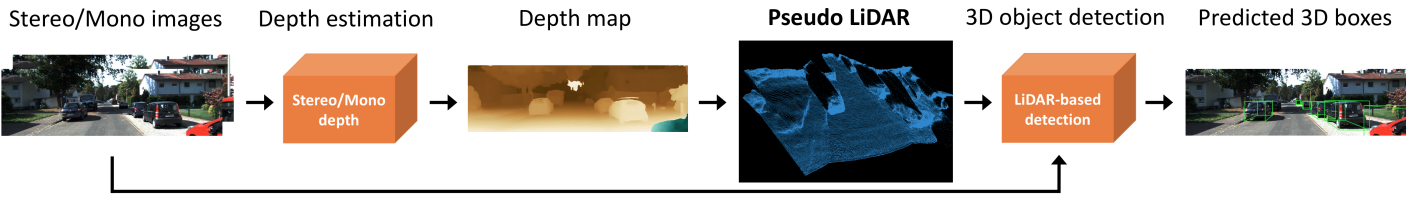
\includegraphics[width=1\textwidth]{../media/wang_pipeline.png}
    \caption{Pipeline of the Pseudo-Lidar estimation network. Stereo (or mono) image data is used to create a disparity map, which is converted to lidar, and is then used by a 3D detector to estimate 3D bounding boxes.}
    \label{wang_pipeline} %label goes last
\end{figure}

In their paper, the authors argue that within a short distance, up to 30 meters away, stereo vision performs competitively with lidar.

\subsection{3D Estimation with Lidar}
Performing 3D estimation and localization with lidar has been a focus for a large portion of the field, and with good reason. Thus, there are many papers which focus on using lidar sensor capabilities to estimate 3D bounding boxes, to varying degrees of success. \cite{qi_frustum_2017} paper, currently one of the best performing networks, forms a part of the work of this research paper as well. 

\subsection{3D Reconstruction with Stereo Data}
\label{sect_reconstruct}
3D reconstruction from a disparity map can be performed multiple similar but slightly different approaches. Regardless of the approach, the goal is to end up with a pointcloud, an unordered set of metric coordinates. The first approach, working with epipolar equations, is the most intuitive. The second, remapping the projected 2D points back into 3D space, is equally effective, but only used to map lidar points onto the image plane (the reverse of reconstruction). \cite{szeliski_computer_2010} goes into some detail over the first method, which principally deals with the high level equations necessary to generate each (x,y,z) coordinate.
\\
\\
\\
The first approach, using epipolar equations, can be described in general as follows. First, some necessary assumptions: 
\begin{itemize} \itemsep=-0.5em
    \item The camera centers are aligned (for simplified rectification).
    \item Images are already rectified (to remove all distortion).
\end{itemize}

There must first be a given disparity map image, $D$, with indices ($u$,$v$) corresponding to the image's x-axis and y-axis (origin located at the top-left of the image). The cameras' intrinsic properties must also be known (P2 for the KITTI dataset), as well as the baseline, $b$, distance (also known as the distance between camera centers). In the KITTI dataset, Camera 2 is the LHS color camera, and thus each record's corresponding P2 matrix is used. The matrix contains the horizontal focal length $f_U$ as well as the vertical focal length $f_V$. \cite{szeliski_computer_2010} describes this in Equation 2.57 of Chapter 2: Image Formation. The camera baseline is given in multiple locations, namely \cite{geiger_are_2012}, although the value is given as "roughly 54 cm", which may reduce the overall accuracy somewhat.

Given this data, the depth value at each pixel location may be calculated via Equation \ref{eq1}, ignoring locations where the disparity value is 0 or Not-A-Number (NaN).
\begin{equation}
z(u,v) = \frac{f_U * b}{D}
\label{eq1}
\end{equation}
Next, the real-world $x$ and $y$ locations may be calculated by taking the relative coordinate location from camera center $(c_U,c_V)$, multiplying by the depth values at each pixel location. Successfully calculating this leads to an estimated metric coordinate value for every valid pixel disparity value in the image.

\begin{equation}
x = \frac{(u - c_U) * z}{f_U}
\end{equation}

\begin{equation}
y = \frac{(v - c_V) * z}{f_V}
\end{equation}

In reality, the calculation is performed in a series of matrix calculations rather than as an element-by-element operation. The "real" steps taken to convert a disparity map into a pointcloud are described in Appendix XX.


% ==============================================================================
\section{Development of 3D Estimation Network}
At this point, we can start talking about how you have modified all the different networks to make them work for you. you should definitely catalog your troubles with each one. we can talk about this in depth. xx

\subsection{Modification of Pyramid Stereo Matching Network}
The first task in creating a network that can take a stereo image pair and generate 3D bounding boxes, as described in figure xx above, is to have the capability of taking a stereo image pair and creating a 2.5D disparity map. To that end, a best-in-class disparity generation algorithm was searched and was selected to be the Pyramid Stereo Matching Network. Pyramid Stereo Matching Network was published by Jia-Ren Chang and Yong-Sheng Chen in March 2018. This network takes a deep learning approach to generating disparity maps from a pair of images. The network itself is near the top of the state of the art, and achieves this by the architecture of its network. (xx architecture and style need to be elaborated upon in the "related work" section). The openly-available repository provided a foundation to start on towards making a compact, easy-to-use function. 

First, the original evaluation code was tested out. Some modification and housekeeping had to be done to ensure that it was compatible with the local installation, as well as being adapted for use with Python 3. All deprecated functionality was manually removed.

\subsubsection{Using a Modified Set of Ground Truths}
After the initial evaluation, the network was prepared for and trained on KITTI data. I first downloaded the network that was pre-trained on the Freiburg SceneFlow dataset, available from the PSMnet authors. Next, I finetuned the network by training it on KITTI data. Here, it must be clarified that there are images in the KITTI stereo dataset that overlap greatly in similarity to those in the KITTI object detection dataset. The difference between the two datasets are essentially that one has been optimized for object detection, and the other for stereo disparity map estimation. This similarity was also noted in [xx], and I took the same approach as [xx authors] to correct it, as described below.Figure xx below also demonstrates the similarity between two sample images, which leads to the problem of having a part of the network trained on what may be validation or even evaluation data. 

\begin{figure}[H]
    \centering  
    \subfigure[000132\_10 from Stereo]{
        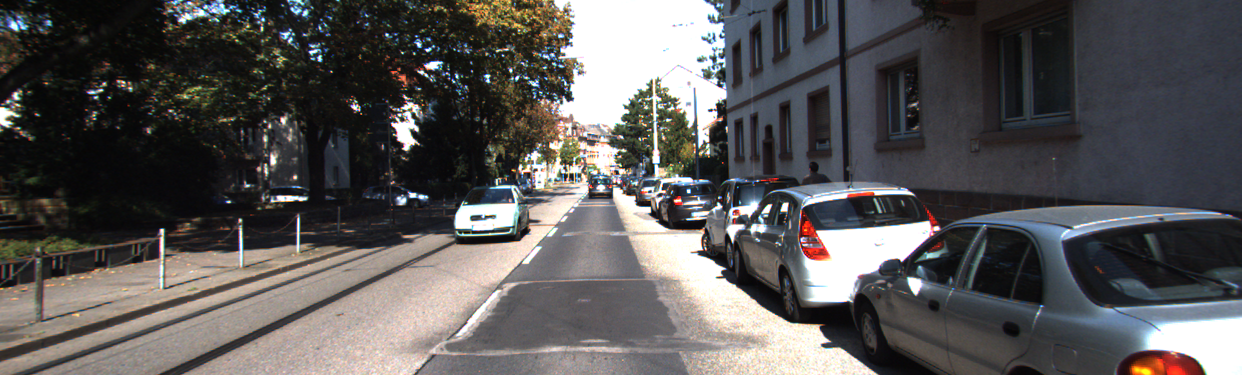
\includegraphics[width=0.485\linewidth]{../media/similar_000132_10_stereo.png}}
    \subfigure[000286 from ObjDet]{
        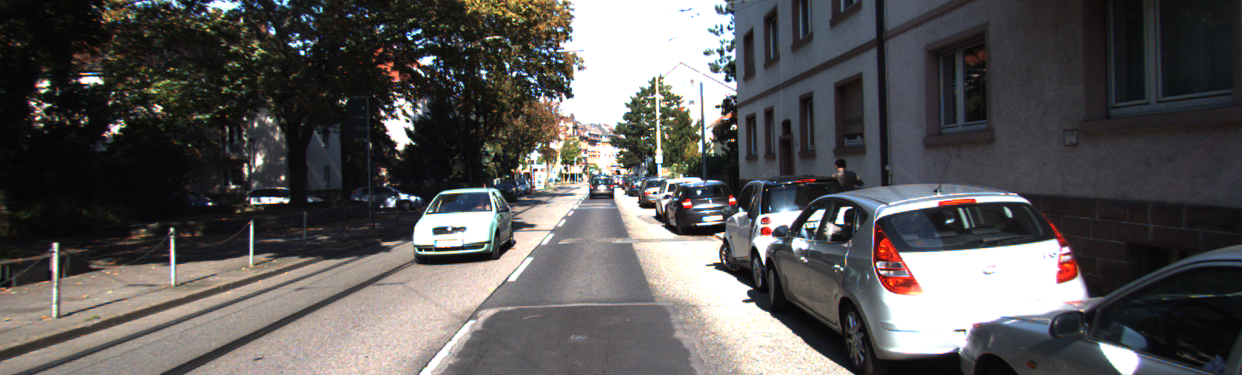
\includegraphics[width=0.485\linewidth]{../media/similar_000286_objdet.png}}
    \label{similarity_stereo_objdet}
    \caption{Example of how two unique records from the separate datasets have overly-similar scenes. There are multiple examples of this, which creates the motivation to generate a secondary set of disparity ground truths for the object detection dataset}
\end{figure}

In order to deal with the dataset overlap, the KITTI object detection dataset was adapted to be used for training stereo data. Lidar data was projected onto the LHS image plane, converted to integer values, then multiplied by a constant. These steps are in line with both the way that [xx] were able to generate their self-made stereo ground truths as well as how the KITTI dataset authors generated their ground truth [xx reference to devkit]. Locations in the image that have no lidar data are left alone at a value of 0.0, and finally the resulting array is saved to a PNG image file format containing integer values. Please refer to the generation script in the repository for the exact steps used to generate the pseudo ground truth stereo images.

\subsection{Development of Stereo 3D Reconstruction Function}
As described in Section \ref{sect_reconstruct}, the overall steps of reconstructing the resulting stereo image consisted of three general equations adapted for use with matrix operations. This also included selecting the proper constants for each calculation. To achieve all this, a specific class was created that would initialize by loading the fully trained model and use it in a non-learning "testing" mode, whereby it would take in either an image path pair or a loaded pair of image arrays. The pair would then be evaluated in PSMnet, which returns a stereo map, and finally be converted to a pointcloud using the epipolar equations in matrix form. Each record of the KITTI dataset has its own calibration file, but the baseline value remained the same. During the overall Frustum Pointnet training and evaluation, a new pointcloud would be generated in real-time.

\subsection{Modification of Frustum Point Net}
Frustum Pointnet, being originally written for Python 2, needed to undergo some minor adaptations while being modified for usage with Python 3. For example, several modules and functions were deprecated or needed modification, and so had to be properly adapted. There are also two actively maintained versions of the frustum Pointnet code. as explained in the original paper [xx], there are two versions of the FPNet model: the first which uses standard Tensorflow libraries, and the second which uses custom Tensorflow operators that must be compiled. For the purposes of this paper, version 1 was used and will be the default version unless otherwise noted. 

In order to transition from using the provided pre-trained model and preprocessed data to self-made preprocessed and trained data, a set of steps and ``paths" were created to guide what was happening in each step and set of ``runs". As shown below in Figure \ref{fp_paths}, there are various steps with gradually increasing dependence on stereo-based pointcloud data. 

\begin{figure}[h] % h = "approx here", {h,t,b}
    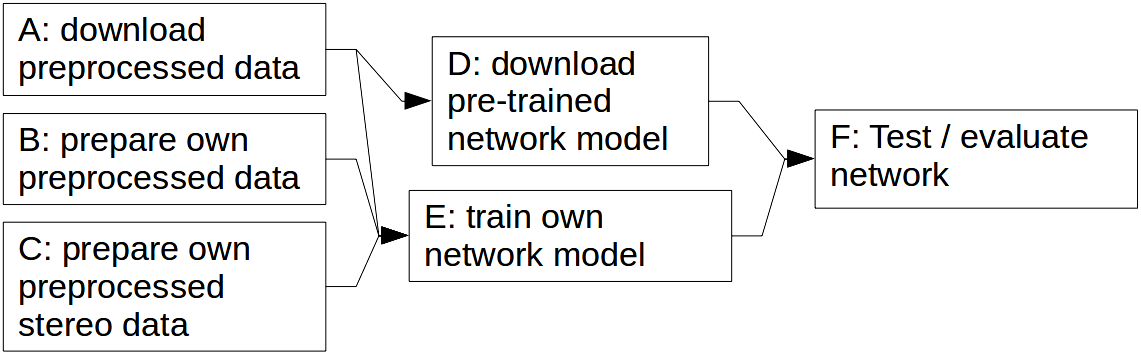
\includegraphics[width=1\textwidth]{../media/fpnet_paths_img.png}
    \caption{Various paths that were planned to simply transition from lidar-based 3D estimation to stereo-based 3D estimation. Generally, paths went chronologically as follow: ADF, AEF, BEF, and finally CEF.}
    \label{fp_paths} %label goes last
\end{figure}

The most basic path, ADF, is simply using the given model to evaluate and achieve similar results to the official paper. Next, AEF used lidar pointclouds, but the model was trained locally. BEF required locally running the "preprocessing" step, but was still theoretically identical to the previous two paths. Finally, CEF truly deviates from 

\section{Procedure / Method}
texthere

\section{Results}
texthere

\section{Conclusion}
